\documentclass[10pt,a4paper]{article}
\usepackage{anysize}
\paperwidth=21cm \paperheight29.7cm
\marginsize{1cm}{1cm}{1cm}{1cm}
\usepackage[utf8]{inputenc}
\usepackage[magyar]{babel}
\usepackage[T1]{fontenc}
\usepackage{amsmath}
\usepackage{amsfonts}
\usepackage{amssymb}
\usepackage{graphicx}
\begin{document}
\title{Méréstechnika laboratórium 2/a jegyzőkönyv}
\author{Koncz István Márton\\\\Neptun: A2754O\\\\Kurzus: TVN2L-D-06\\\\Mérésvezető: Markella Zsolt\\\\B csoport}
\date{\today}
\maketitle
\newpage
\section{12. sz. laboratóriumi mérés}
	Mérés dátuma:\date{2017.09.18}
	\subsection{A mérés célja}
	A teljesítmény összetevőinek, jellemzőinek méréssel történő meghatározása.
A mérés hibáinak meghatározása, figyelembevétele.
	\subsection{Mérési feladatok}
		\subsubsection{A mérőpanelen található izzó teljesítmény-feszültség karakterisztikájának meghatározása! A teljesítménymérő
használatának megismerése.
A teljesítmény számítása ill. mérése hibáinak
meghatározása!}
Cél: A mérőpanelen található $24 V$, $60 W$-os izzó a
teljesítmény mérése teljesítménymérővel valamint
teljesítmény-feszültség karakterisztikájának
felvétele, váltakozó feszültségű táplálás esetén, $0$ –
$20 V$ tartományban $2 V$-os lépésenként.\\\\
A mérendő objektum:\begin{figure}[hbtp]
\centering
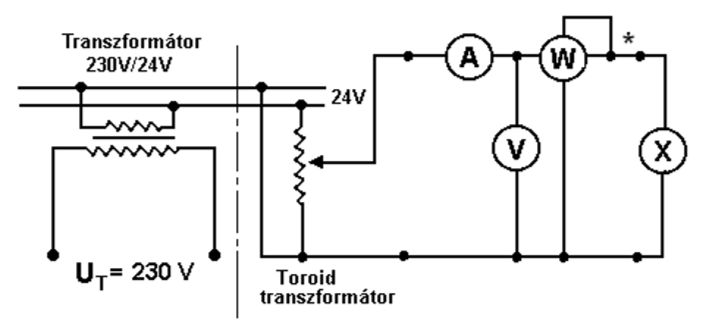
\includegraphics[scale=0.5]{Toroid.png}
\caption{}
\end{figure}
$$$$
Mérés határadatai: a megengedett áram és feszültség $2 A$, $20 V$.
$$$$
$U_T$: tápfeszültség\\\\
$U_M$: izzón eső feszültség\\\\
$I_M$: izzón folyó áram\\\\
$P_M$: izzó teljesítménye\\\\
\newpage
\begin{table}


\centering
\begin{tabular}{|c|c|c|c|c|}

\hline 
$U_T$  & $U_M$ & $I_M$ & $P_M$ & $R_{SZ}$ \\ 
\hline 
0 V & 0,001 V & 0,02 A & 0,04 W & ~ 0 $\Omega$ \\ 
\hline 
2 V & 1,9 V & 0,68 A & 1,43 W & 2,79 $\Omega$ \\ 
\hline 
4 V & 3,7 V & 0,93 A & 3,79 W & 3,97 $\Omega$ \\ 
\hline 
6 V & 5,65 V & 1,13 A & 7,08 W & 5 $\Omega$ \\ 
\hline 
8 V & 7,8 V & 1,33 A & 10,51 W & 5,86 $\Omega$ \\ 
\hline 
10 V & 9,78 V & 1,47 A & 15 W & 6,65 $\Omega$ \\ 
\hline 
12 V & 11,76 V & 1,62 A & 19,37 W & 7,25 $\Omega$ \\ 
\hline 
14 V & 13,71 V & 1,76 A & 24,36 W & 7,78 $\Omega$ \\ 
\hline 
16 V & 15,7 V & 1,89 A & 30,4 W & 8,3 $\Omega$ \\ 
\hline 
\end{tabular} 
\end{table}
$18V$ és $20V$ esetén átlépnénk a $2A$-es áramkorlátot, ezért a mérést ezekben a tartományokban nem végeztem el. \\\\
\begin{figure}[hbtp]
			 \centering
			 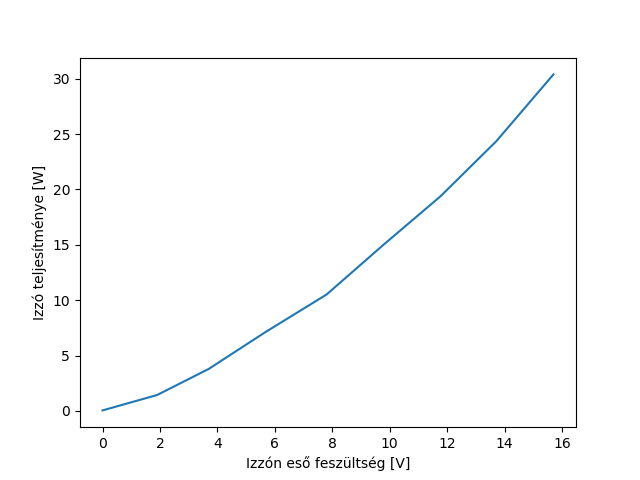
\includegraphics[scale=0.7]{telj_fesz.png}
			 \caption{Izzó teljesítménye a feszültség függvényében}
			 \end{figure}\\\\
			 \begin{figure}[hbtp]
			 \centering
			 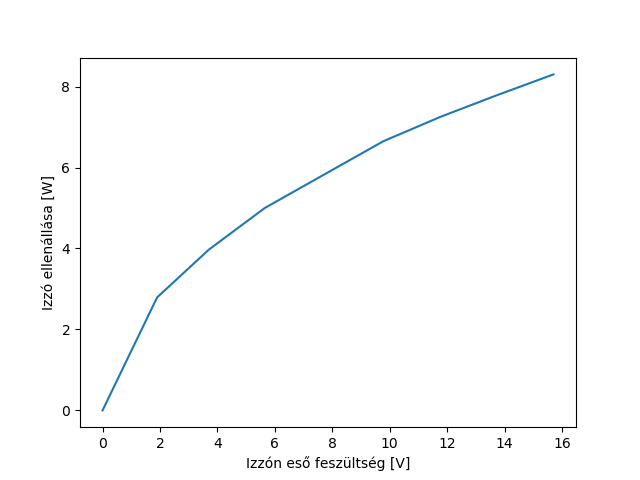
\includegraphics[scale=0.7]{ell_fesz.png}
			 \caption{Izzó ellenállása a feszültség függvényében}
\end{figure}
\newpage
Áramot MAXWELL MX-25 201 multiméterrel mértem, amelynek a bizonytalansági mutatói a következők 20 A méréshatáron (váltakozó áram esetén): $$\pm h = \pm 3.0\% rdg + 10 digit$$
Számítás:
$$\pm h_{I1} = \pm \left(3 + \frac{10}{68} * 100\right) \% = \pm 17.7 \% $$
$$\pm h_{I2} = \pm \left(3 + \frac{10}{93} * 100\right) \% = \pm 13.7 \% $$
$$\pm h_{I3} = \pm \left(3 + \frac{10}{113} * 100\right) \% = \pm 11.8 \% $$
$$\pm h_{I4} = \pm \left(3 + \frac{10}{133} * 100\right) \% = \pm 10.5 \% $$
$$\pm h_{I5} = \pm \left(3 + \frac{10}{147} * 100\right) \% = \pm 9.8 \% $$
$$\pm h_{I6} = \pm \left(3 + \frac{10}{162} * 100\right) \% = \pm 9.1 \% $$
$$\pm h_{I7} = \pm \left(3 + \frac{10}{176} * 100\right) \% = \pm 8.6 \% $$
$$\pm h_{I8} = \pm \left(3 + \frac{10}{189} * 100\right) \% = \pm 8.3 \% $$

Feszültséget HAMEG HM8012 multiméterrel mértem, amelynek a bizonytalansági mutatói a következők $50 V$ méréshatáron (váltakozó áram esetén):
$$\pm h = \pm 0.07\% fs + 0.4 \% rdg$$
Számítás:
$$\pm h_{U1} = \pm \left(0.4 + \frac{50}{1.9} * 0.07\right) \% = \pm 2.2 \%$$
$$\pm h_{U2} = \pm \left(0.4 + \frac{50}{3.7} * 0.07\right) \% = \pm 1.3 \%$$
$$\pm h_{U3} = \pm \left(0.4 + \frac{50}{5.65} * 0.07\right) \% = \pm 1.01 \%$$
$$\pm h_{U4} = \pm \left(0.4 + \frac{50}{7.8} * 0.07\right) \% = \pm 0.84 \%$$
$$\pm h_{U5} = \pm \left(0.4 + \frac{50}{9.78} * 0.07\right) \% = \pm 0.75 \%$$
$$\pm h_{U6} = \pm \left(0.4 + \frac{50}{11.76} * 0.07\right) \% = \pm 0.69 \%$$
$$\pm h_{U7} = \pm \left(0.4 + \frac{50}{13.71} * 0.07\right) \% = \pm 0.65 \%$$
$$\pm h_{U8} = \pm \left(0.4 + \frac{50}{15.7} * 0.07\right) \% = \pm 0.62 \%$$

A teljesítmény hibája a mért feszültség, illetve áramértékek hibáinak összege, mivel $P = U * I$,
(ahol $P$ a teljesítmény, $U$ a feszültség, és $I$ az áramerősség)
$$\pm h_{P1} = \pm \left(h_{I1} + h_{U1}\right) \% = \pm \left(17.7 + 2.2\right) \% = \pm 19.9 \%$$
$$\pm h_{P2} = \pm \left(h_{I2} + h_{U2}\right) \% = \pm \left(13.7 + 1.3\right) \% = \pm 15 \%$$
$$\pm h_{P3} = \pm \left(h_{I3} + h_{U3}\right) \% = \pm \left(11.8 + 1.01\right) \% = \pm 12.81 \%$$
$$\pm h_{P4} = \pm \left(h_{I4} + h_{U4}\right) \% = \pm \left(10.5 + 0.84\right) \% = \pm 11.34 \%$$
$$\pm h_{P5} = \pm \left(h_{I5} + h_{U5}\right) \% = \pm \left(9.8 + 0.75\right) \% = \pm 10.55 \%$$
$$\pm h_{P6} = \pm \left(h_{I6} + h_{U6}\right) \% = \pm \left(9.1 + 0.69\right) \% = \pm 9.79 \%$$
$$\pm h_{P7} = \pm \left(h_{I7} + h_{U7}\right) \% = \pm \left(8.6 + 0.65\right) \% = \pm 9.25 \%$$
$$\pm h_{P8} = \pm \left(h_{I8} + h_{U8}\right) \% = \pm \left(8.3 + 0.62\right) \% = \pm 8.92 \%$$
\newpage
			 \subsubsection{Teljesítmény mérés ohmos-induktív terhelés esetén}
A mérés során egy, az ohmos terheléssel (izzóval) sorosan kapcsolt tekercs hatását mérjük, úgy, hogy a vasmag kiszerelhetőségének segítségével változtatjuk a tekercs induktivitását.
A teljesítménymérővel a hatásos teljesítményt mérünk.
\\\\
A mérendő objektum:\begin{figure}[hbtp]
\centering
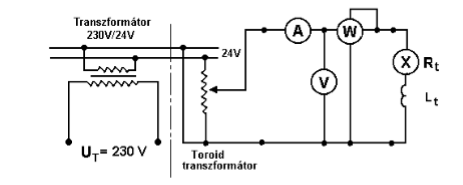
\includegraphics[scale=1]{ohm_tekercs.png}
\caption{}
\end{figure}
\\\\ Mért eredmények:$$$$
\begin{tabular}{|c|c|c|c|c|c|c|}
\hline 
Módszer & $U_T$ & $I_M$ & $U_M$ & $P_M$ & $Q_M$ & $S_M$ \\ 
\hline 
Vasmag nélkül & 5 V & 1,03 A & 5,11 V & 5,23 W & 0,18 VAr & 5,23 VA \\ 
\hline 
 & 10 V & 1,46 A & 10,19 V & 14,85 W & 0,37 VAr & 14,85 VA \\ 
\hline 
Vasmaggal & 5 V & 0,53 A & 5,09 V & 2,25 W & 1,48 VAr & 2,69 VA \\ 
\hline 
 & 10 V & 0,85 A & 10,1 V  & 7,5 W & 3,81 VAr & 8,1 VA \\ 
\hline 
Gumilappal a vasmag résében & 5 V & 1 A & 5,19 V & 4,93 W & 1,14 VAr & 5,06 VA \\ 
\hline 
 & 10 V & 1,44 A & 10,23 V  & 14,31 W & 2,41 VAr & 14,52 VA \\ 
\hline 
\end{tabular} 
$$$$
Számítások:
\begin{enumerate}
	\item Vasmag nélkül:
		\begin{itemize}
			\item[--] 5V:
			$$S = U * I$$
			$$S_{sz} = 5,11 V * 1,03 A =5,26 VA $$
			$$\frac{P}{\left|S\right|} = \cos^{-1} \phi = \frac{5,23 W}{5,26 VA} = 0,9942$$
			$$\phi = 6,122$$
			$$Q_{sz} = \sin \phi *\left|S\right| = 0,56 VAr$$
			\item[--] 10V:
			$$S = U * I$$
			$$S_{sz} = 10,19 V * 1,46 A =14,87 VA $$
			$$\frac{P}{\left|S\right|} = \cos^{-1} \phi = \frac{14,85 W}{14,87 VA} = 0,9986$$
			$$\phi = 2,971$$
			$$Q_{sz} = \sin \phi *\left|S\right| = 0,77 VAr$$
		\end{itemize}
		\newpage
		\item Vasmaggal:
		\begin{itemize}
			\item[--] 5V:
			$$S = U * I$$
			$$S_{sz} = 5,09 V * 0,53 A =2,69 VA $$
			$$\frac{P}{\left|S\right|} = \cos^{-1} \phi = \frac{2,25 W}{2,69 VA} = 0,8364$$
			$$\phi = 33,23$$
			$$Q_{sz} = \sin \phi *\left|S\right| = 1,47 VAr$$
			\item[--] 10V:
			$$S = U * I$$
			$$S_{sz} = 10,1 V * 0,85 A =8,585 VA $$
			$$\frac{P}{\left|S\right|} = \cos^{-1} \phi = \frac{7,5 W}{8,585 VA} = 0,8736$$
			$$\phi = 29,118$$
			$$Q_{sz} = \sin \phi *\left|S\right| = 4,1775 VAr$$
		\end{itemize}
		\item Gumilappal a vasmag résében:
		\begin{itemize}
			\item[--] 5V:
			$$S = U * I$$
			$$S_{sz} = 5,19 V * 1 A =5,19 VA $$
			$$\frac{P}{\left|S\right|} = \cos^{-1} \phi = \frac{4,93 W}{5,19 VA} = 0,9499$$
			$$\phi = 18,21$$
			$$Q_{sz} = \sin \phi *\left|S\right| = 1,62 VAr$$
			\item[--] 10V:
			$$S = U * I$$
			$$S_{sz} = 10,23 V * 1,44 A =14,73 VA $$
			$$\frac{P}{\left|S\right|} = \cos^{-1} \phi = \frac{14,31 W}{14,73 VA} = 0,9714$$
			$$\phi = 13,715$$
			$$Q_{sz} = \sin \phi *\left|S\right| = 3,49 VAr$$
		\end{itemize}
\end{enumerate}
\newpage
\begin{figure}[hbtp]
\centering
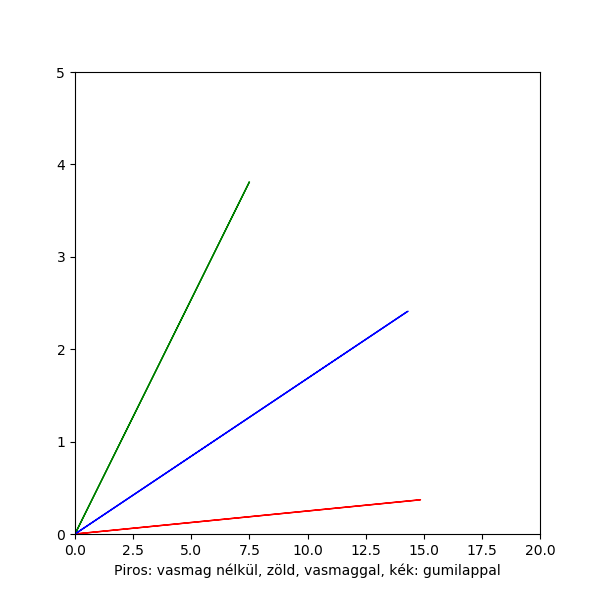
\includegraphics[scale=1]{vektor.png}
\caption{Vektorábra 10 V-os tápfeszültség esetén}
\end{figure}
	\subsubsection{Pákatranszformátor kimeneti jellegörbéjének felvétele}
	Számítsa ki a mérőhelyen található $20 VA$-s pákatranszformátor $24 V$-s
kimenetére vonatkozó névleges terhető áram és terhelő ellenállás értékét. Mérje
meg a pákatranszformátor $24 V$-s kimenetének üresjárási feszültségét! A
mellékelt tolóellenállás felhasználásával állítsa be a névleges terhelő áramot és
ismételje meg az előző mérést! A mért értékek alapján számítsa ki a
feszültségesés illetve a teljesítmény veszteség értékét. A mérés eredményét
ábrázolja $U_{ki}$, $I_{Ki}$ koordinátarendszerben.
\\\\
A mérés határadatai: 
\\\\Névleges teljesítmény: $$P_N = 20 VA$$
Névleges áram: $$I_N = \frac{P_N}{U} = \frac{20 VA}{24 V} = 0,83 A$$
\newpage
\section{13. sz. laboratóriumi mérés}
	Mérés dátuma:\date{2016.09.13}
	\subsection{A mérés célja}
	A digitális oszcilloszkóp kezelésének többlet funkcióinak
elsajátítása, a kapott mérési eredmények kiértékeléséhez
szükséges szemlélet kialakítása.
	\subsection{Mérési feladatok}
		\subsubsection{Az oszcilloszkóp csatorna-menük vizsgálata}
		\begin{enumerate}
			\item Beállítások változtatásának eredményei CH1 csatornán:
				\begin{itemize}
					\item[--] Csatolás: nincs változás, akkor lenne, ha ténylegesen jelet kötnénk a bemenetre
					\item[--] Sávkorlátozás: V/DIV kijelzésnél megjelenik egy BW felirat, ha be van kapcsolva
					\item[--] V/DIV: pontosabb beállítás
				\end{itemize}
			\item Az 1V/DIV és a 10mV/DIV finom-beállítások közötti eltérések:\\\\
			\begin{tabular}{|c|c|}
			\hline 
			1V/DIV & 10mV/DIV \\ 
			\hline 
			2V<X<5V: 40mV & 10mV<X<11mv: 0,2mV \\ 
			\hline 
			1V<X<2V: 20mV & 5mV<X<10mV: 0,1mV \\ 
			\hline 
			500mV<X<1V: 10mV & - \\ 
			\hline 
			\end{tabular}
			\item A függőleges pozíció állításához tartozó megfigyeléseim:
				\begin{itemize}
					\item[--] CH1 csatorna függőleges pozíciója 1 osztással feljebb került +100mV esetén
					\item[--] -150mV pozíció mellett a lépésköz 4mV
				\end{itemize}				 
		\end{enumerate}
		\subsubsection{Horizontális menü vizsgálata}
		\begin{enumerate}
			\item A Window megjelenítés hatása, rajzzal:
			\\\\
						\begin{figure}[hbtp]
						\centering
				    		 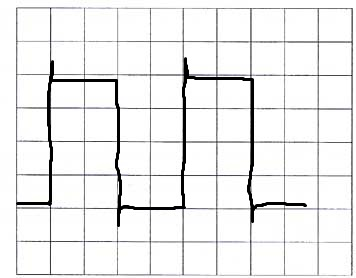
\includegraphics[scale=0.5]{teljes/osc_hor.jpg}
						\caption{Ablaktartomány beállításakor}
						\end{figure}
			\\
					\begin{figure}[hbtp]
					\centering
					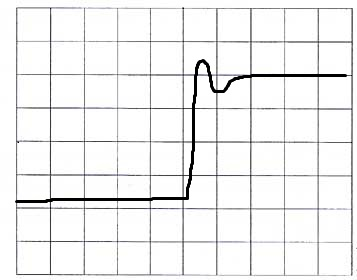
\includegraphics[scale=0.5]{teljes/osc_hor_zoom.jpg}
					\caption{Ablak megjelenítésekor}
					\end{figure}\\\\
			\item Sec/DIV hatása: Belenagyítunk a képbe.
			\item Autoset hatása, rajzzal:
			Autoset hatására az ábra értékelhetetlen. A megállításhoz szükséges holdoff idő: $6,950 \mu s$ \\\\\begin{figure}[hbtp]
			\centering
			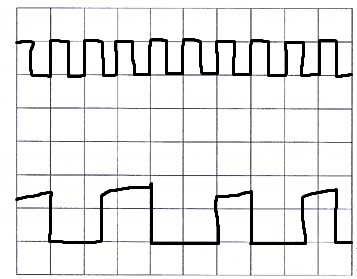
\includegraphics[scale=0.5]{teljes/osc_autoset.jpg}
			\caption{Autoset}
			\end{figure}
					
		\end{enumerate}
		\subsubsection{Az utótriggerelés, az előtriggerelés és a késleltetett utótriggerelés vizsgálata}
			\begin{enumerate}
				\item A vízszintes pozíció állító működésének vizsgálata:\\
				-1 osztással való trigger pozíció állítás 90 fokos fáziskését jelent.	A +5 DIV-es eltolás egy előző egész periódust jelenít meg a képernyő közepétől. A nagy tartományban való állíthatóság jól használható a trigger pozíció előtti vagy utáni jelalak  vizsgálatára.
				\item Set to Zero vizsgálata: a gomb megnyomásával a képernyő közepére helyezhetjük a trigger pozíciót.
				\item Az oszcilloszkóp jelalakjainak vizsgálata:
				\\\\
				\begin{figure}[hbtp]
				\centering
				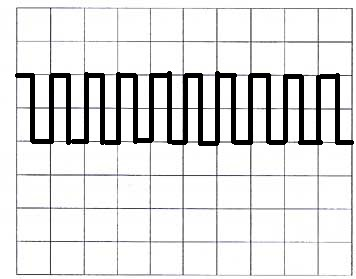
\includegraphics[scale=1]{teljes/osc_Qa_1.jpg}
				\caption{1MHz négyszögjel}
				\end{figure}
				\begin{figure}[hbtp]
				\centering
				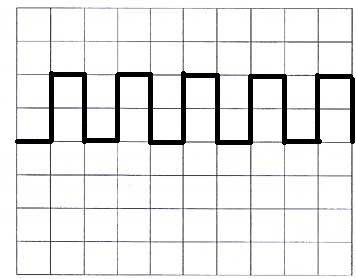
\includegraphics[scale=1]{teljes/osc_Qa_2.jpg}
				\caption{QA}
				\end{figure}
				\begin{figure}[hbtp]
				\centering
				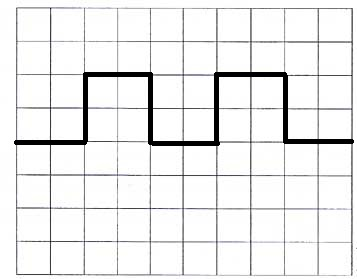
\includegraphics[scale=1]{teljes/osc_Qa_3.jpg}
				\caption{QB}
				\end{figure}
				\begin{figure}[hbtp]
				\centering
				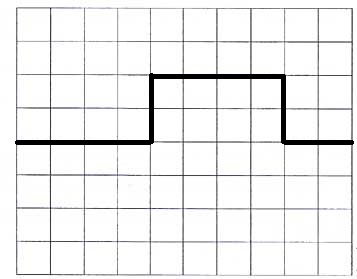
\includegraphics[scale=1]{teljes/osc_Qa_4.jpg}
				\caption{QC}
				\end{figure}
				\begin{figure}[hbtp]
				\centering
				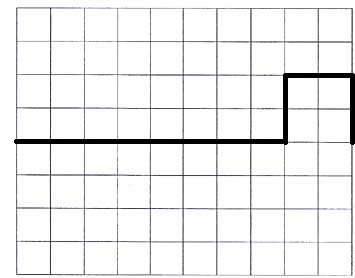
\includegraphics[scale=1]{teljes/osc_Qa_5.jpg}
				\caption{QD}
				\end{figure}
				\item A jel a képernyőn kívüli részeinek vizsgálata: késleltetett utótriggerelési mód. A memória mérete korlátozza a feldolgozható adatmennyiséget.
			\end{enumerate}
			\subsubsection{A trigger menü vizsgálata}
			\begin{enumerate}
				\item Nagy és kisfrekvenciás elnyomás határfrekvenciájának mérése.\\\\\begin{tabular}{|c|c|}
				\hline 
				Triggerforrás & CH1 \\ 
				\hline 
				Trigger él & emelkedő \\ 
				\hline 
				Triggerelési üzemmód & Auto \\ 
				\hline 
				Triggerjel csatolása & HF: 55 kHz; LF: 13,52 kHz \\ 
				\hline 
				\end{tabular}$$$$
				Lépések: A trigger jelet csatlakoztatjuk. A trigger menüben éltrigger módot választjuk ki, majd a csatolás típusát HF reject-re állítjuk. Ezzel leválasztjuk a nagyfrekvenciás komponenseket. Két lehetőségünk adódik:
				\begin{enumerate}
					\item Megvizsgáljuk a jel spektrumát FFT-vel.
					\item A triggerjel frekvenciáját változtatjuk és vizsgáljuk a jel szintjét. Amikor a jel $3 dB$-el lecsökken a középfrekvenciához képest, akkor az lesz a határfrekvencia.
					
				\end{enumerate}				   
				\item 1 kHz-es négyszögjel vizsgálata CH1 csatornán, kb. 500 $\mu s$ impulzusszélesség mellett: alsó határ 481 $\mu s$, felső határ 532 $\mu s$
			\end{enumerate}
			\subsubsection{Kibővített matematikai funkciók vizsgálata}
			A Math Menu gomb 3 funkciót kínál: összegzés, különbségképzés, FFT spektrum analízis.
			\subsubsection{Automatikus gyorsmérések elvégzése}
			\begin{tabular}{|c|c|c|}
			\hline 
			Mennyiség & Szinuszjel & Négyszögjel \\ 
			\hline 
			f & $1 kHz$ & $10 kHz$ \\ 
			\hline 
			T & $1 ms$ & $100 \mu s$ \\ 
			\hline 
			Mean & $23,7 mV$ & $134 mV$ \\ 
			\hline 
			Pk-Pk & $3,92 V$ & $2,72 V$ \\ 
			\hline 
			Cyc RMS & $1,37 V$ & $1,10 V$ \\ 
			\hline 
			Min & $-1,92 V$ & $-1,04 V$ \\ 
			\hline 
			Max & $2,0 V$ & $1,32 V$ \\ 
			\hline 
			Rise time & $296 \mu s$ & $79,6 ns$ \\ 
			\hline 
			Fall time & $288 \mu s$ & $78,57 ns$ \\ 
			\hline 
			Pos Width & $494 \mu s$ & $50,67 \mu s$ \\ 
			\hline 
			Neg Width & $506 \mu s$ & $49,40\mu s$ \\ 
			\hline 
			\end{tabular} 
			$$$$
			Négyszögjel felfutási idejének mérése:\\\\
			\begin{tabular}{|c|c|}
			\hline 
			TIME/DIV & Négyszögjel felfutási ideje \\ 
			\hline 
			$50 \mu s$ & $157 ns$ \\ 
			\hline 
			$25 \mu s$ & $76,79 \mu s$ \\ 
			\hline 
			$10 \mu s$ & $33,85 \mu s$ \\ 
			\hline 
			$5\mu s$ & $28,75 \mu s$ \\ 
			\hline 
			\end{tabular} 
\section{14. sz. laboratóriumi mérés}
	Mérés dátuma:\date{2016.10.04}
	\subsection{A mérés célja}
	Az ellenállás mérésére használatos néhány módszer alkalmazásának elsajátítása. Igen kis ellenállások nagypontosságú mérése.
A méréseknél előforduló mérési hibák meghatározása.
	\subsection{Mérési feladatok}
		\subsubsection{Feszültség összehasonlító módszerrel határozza meg a 4. sz
mérőpanelen található R7 $= 10 \Omega $ és R4 $= 82 \Omega $ névleges értékű ellenállások pontos értékét és bizonytalanságukat!
A mért és a számított eredményeket foglalja össze táblázatba. A méréseknél
az elérhető legnagyobb pontosságra törekedjék!}
		Mérendő objektum:
		\\\\
		\begin{figure}[hbtp]
		\centering
		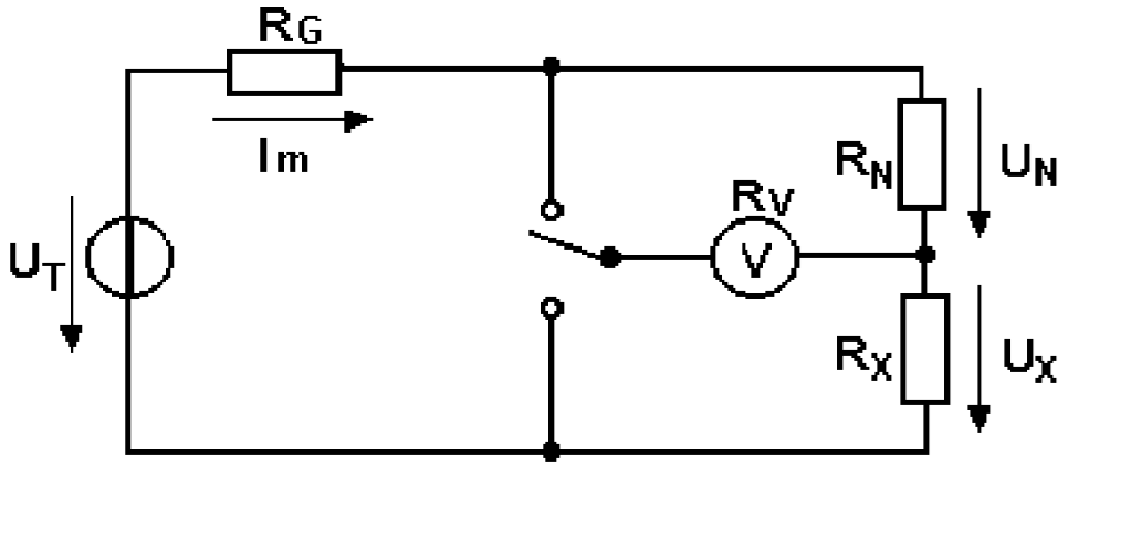
\includegraphics[scale=0.5]{teljes/fesz_ossze.png}
		\caption{Feszültség összehasonlító módszer}
		\end{figure}
		\\\\
		Határadatok: mivel $R_G$ a legnagyobb ellenállás, és mindegyiknek a megengedett maximálisan felvehető teljesítménye $0,25 W$, ezért célszerű $R1 = R_G$ ellenállással a maximális tápfeszültséget meghatározni.
		$$P = I^2_{m} * R$$
		$$I_m = \sqrt{\frac{P}{R}} = \sqrt{\frac{0,25W}{1k\Omega}} = 15,8 mA$$
		$$U_{Tmax} = \frac{I_m * R_G}{3} = \frac{15,8 mA * 1 k\Omega}{3} = 5 V$$
		Mért értékek:\\\\
		\begin{tabular}{|c|c|c|}
		\hline 
		$R_x$ & $R_4$ & $R_7$ \\ 
		\hline 
		$U_N$ & 45,93 mV & 43,57 mV \\ 
		\hline 
		$U_X$ & 47,97 mV & 368 mV \\ 
		\hline 
		$R_{valodi}$ & 10,44 $\Omega$ & 84,46 $\Omega$ \\ 
		\hline 
		\end{tabular} 
		$$R_X = R_N * \frac{U_X}{U_N}$$
		
		Hibaszámítás (HM8012):\\\\
		$$\pm h_u = \pm \left(0,05\% + 0,004\% * \frac{U_{mh}}{U_m}\right)$$
		\begin{enumerate}
			\item $R_4$:
			$$\pm h_{UR4} = \pm \left(0.05 + 0.004*\frac{500 mV}{47,97 mV}\right) \% = \pm 0,091 \% $$
			$$\pm h_{URN} = \pm \left(0.05 + 0.004*\frac{500 mV}{45,93 mV}\right) \% = \pm 0,093 \% $$
			$$\pm h_{RN} = \pm 0.02 \%$$
			$$\pm h_{RX} = \pm \left(h_{UR4} + h_{URN} + h_{RN}\right) \% = \pm 0,204 \%$$
			\item $R_7$:
			$$\pm h_{UR7} = \pm \left(0.05 + 0.004*\frac{500 mV}{43,57 mV}\right) \% = \pm 0,095 \% $$
			$$\pm h_{URN} = \pm \left(0.05 + 0.004*\frac{500 mV}{45,93 mV}\right) \% = \pm 0,055 \% $$
			$$\pm h_{RN} = \pm 0.02 \%$$
			$$\pm h_{RX} = \pm \left(h_{UR4} + h_{URN} + h_{RN}\right) \% = \pm 0,17 \%$$
		\end{enumerate}
		
		
		\subsubsection{Áramösszehasonlító módszerrel határozza meg a 4. sz mérőpanelen
található R15 $= 100 k\Omega$ névleges értékű, valamint az R11 ismeretlen értékű
ellenállásokat és bizonytalanságukat! A mért és a számított eredményeket
foglalja össze táblázatba. A méréseknél az elérhető legnagyobb pontosságra
törekedjék!
}		Mérendő objektum:
		\\\\\begin{figure}[hbtp]
		\centering
		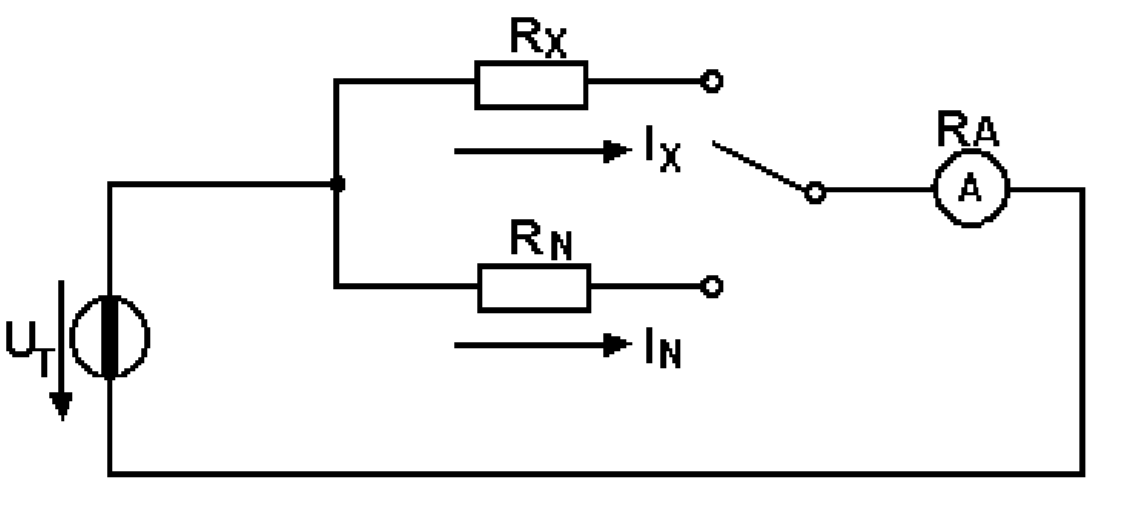
\includegraphics[scale=0.2]{teljes/aram_ossze.png}
		\caption{Áram összehasonlító módszer}
		\end{figure}
		\\\\Határadatok: Áramkorlát $I = 3mA$, feszültségkorlát:$$
		P= U*I$$
		$$U_{max} = \sqrt{P*R} = \sqrt{0,25 * 100 k\Omega} = 158V$$
		$$U_T = \frac{U_{max}}{5} = 30 V $$
		\\\\Mért értékek:\\\\
		\begin{tabular}{|c|c|c|}
		\hline 
		$R_x$ & $R_{11}$ & $R_{15}$ \\ 
		\hline 
		$I_N$ & $300 \mu A$ & $300 \mu A$ \\ 
		\hline 
		$I_X$ & $844 \mu A$ & $303,6 \mu A$ \\ 
		\hline 
		$R_{valodi}$ & $35,54 k\Omega$  & $98,82 k\Omega$ \\ 
		\hline 
		\end{tabular}
		$$R_X = R_N * \frac{I_N}{I_X}$$ 
		Hibaszámítás (Maxwell):
		$$\pm h = \pm \left(h_{rdg} + \frac{D}{N_K}*100\right) \%$$
		\begin{enumerate}
			\item $R_{11}$:
			$$\pm h_{IN} = \pm \left(h_{rdg} + \frac{D}{N_K}*100\right) = \pm 1,83 \%$$
		\end{enumerate}
		
		$$\pm h_{IR11} = \pm 1,61 \%$$
		$$\pm h_{IR15} = \pm 1,83 \%$$
		$$\pm h_{RX} = \pm \left(h_{RN} + h_{IN} + h_{IX}\right)$$
		$$\pm h_{R11} = \pm 3,46 \%$$
		$$\pm h_{R15} = \pm 3,68 \%$$
		\newpage
		\subsection{Két- ill. négyvezetékes módszer segítségével határozza meg a 4. sz
mérőpanelen található R3 =$ 0,5\Omega$ névleges értékű ellenállást! A mért és a
számított eredményeket foglalja össze táblázatba A méréseknél az elérhető
legnagyobb pontosságra törekedjék!}
		Mérendő objektum:\\\\
		\begin{figure}[hbtp]
		\centering
		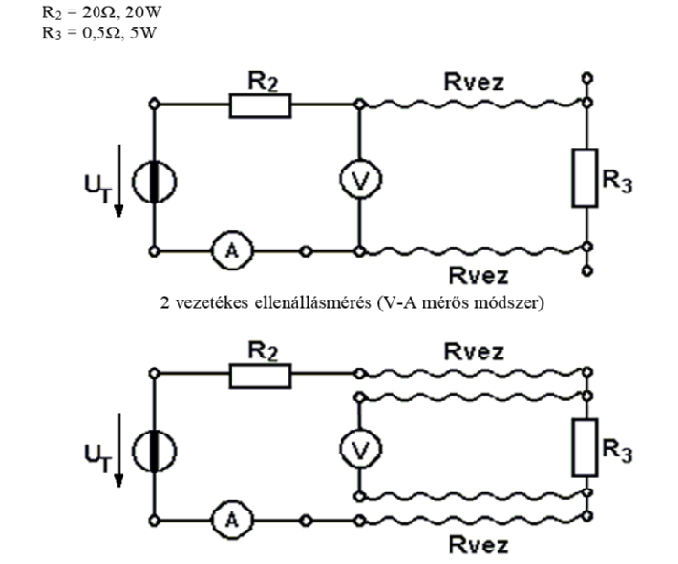
\includegraphics[scale=0.5]{teljes/ket_negy_vez.png}
		\caption{4 vezetékes ellenállásmérés}
		\end{figure}
		
		Határadatok:
		$$I = \sqrt{\frac{P_{R2}}{R_2}} I = \sqrt{\frac{20W}{20\Omega}} = 1 A$$
		$$U_T = I * \left(R2 + R3\right) = 1A * \left(20\Omega + 0,5\Omega\right) = 20,5 V$$\begin{tabular}{|c|c|c|c|}
		\hline 
		Módszer & I & U & R \\ 
		\hline 
		Kétvezetékes rövid & 0,9 mA & 504 mV & $0,561 \Omega$ \\ 
		\hline 
		Kétvezetékes hosszú & 0,9 mA & 587 mV & $0,652 \Omega$ \\ 
		\hline 
		Négyvezetékes rövid & 0,9 & 472 mV & $0,524 \Omega$ \\ 
		\hline 
		Négyvezetékes hosszú & 0,9 & 491 mV & $0,545 \Omega$ \\ 
		\hline 
		\end{tabular} 
		\newpage
\section{15. sz. laboratóriumi mérés}
	Mérés dátuma:\date{2016.09.27}
	\subsection{A mérés célja}
	Kapuzással és impulzusszámlálással dolgozó digitális frekvencia- és időmérő
működési elvének és működésének modellen történő bemutatása az alapvető
üzemmódokban. A kapcsolást alkotó áramkörök vizsgálata.

	\subsection{Mérési feladatok}
		\subsubsection{Az Nx számláló számlálási bizonytalanságának mérése}
		Állítson be a függvénygenerátoron kb. 15Hz-es négyszög-jelet! Válasszon a
mérőpanel frekvenciamérő üzemmódjában 10MHz-es méréshatárt és mérje
meg a jel frekvenciáját!
		\begin{figure}[hbtp]
		\centering
		\includegraphics[scale=0.5]{teljes/nx_biz.png}
		\caption{Az impulzusszámlálás hibája}
		\end{figure}
		\subsubsection{Közvetlen frekvenciamérés}
		Oszcilloszkóp segítségével állítson be a függvénygenerátor kimenetén
négyszögjelet, a pozitív szint 3 V, a negatív szint 0 V legyen!
		\\\\
		Mérendő objektum:
		\begin{figure}[hbtp]
		\centering
		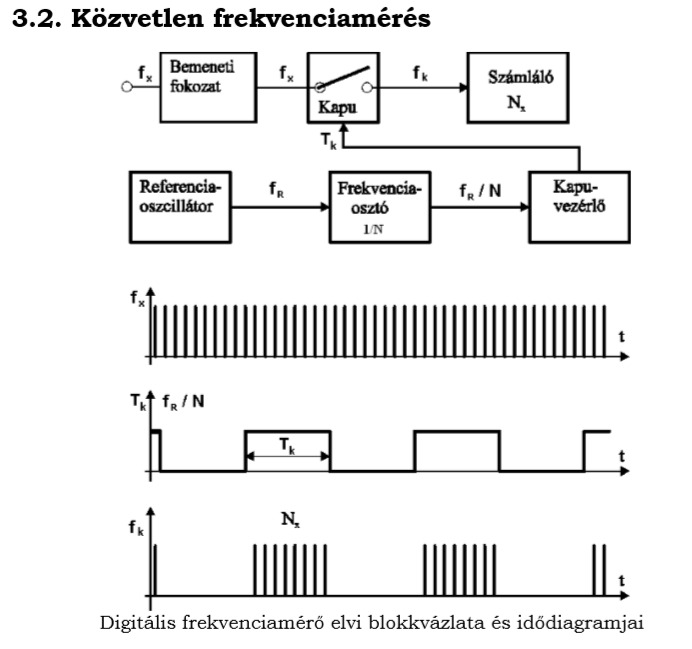
\includegraphics[scale=0.3]{teljes/kozv_frekvencia.png}
		\caption{}
		\end{figure}
		\newpage\begin{tabular}{|c|c|c|c|c|c|c|}
		\hline 
		f[Hz] & 10 & $10^2$ & $10^3$ & $10^4$ & $10^5$ & $10^6$ \\ 
		\hline 
		Nx & 1 & 10 & 103 & 1040 & 10083 & 100325 \\ 
		\hline 
		$h_{fx}$ & 1 & 0,1 & 0,01 & 0,001 & 0,0001 & 0,00001 \\ 
		\hline 
		\end{tabular} 
		$$h_{fx} = h_{fR} + \frac{1}{Nx}; h_{fR} = 10^{-6}$$
		$$Mode=FREQ; RANGE=10000 \frac{kHz}{ms}$$
		RANGE kapcsoló 3 állásának mérése:\\\\
		\begin{tabular}{|c|c|c|c|}
		\hline 
		RANGE & 100 kHz & 1000 kHz & 10000 kHz \\ 
		\hline 
		Nx & 10029 & 10029 & 1003 \\ 
		\hline 
		$h_{fX}$ & 0,00010071 & 0,00010071 & 0,000998008 \\ 
		\hline 
		\end{tabular} 
		\\\\A RANGE kapcsoló legnagyobb állásában a hiba 10x-sére nőtt, mivel nem elég digit a kijelzéshez.
		\subsubsection{Periódusidőmérésen alapuló frekvenciamérés}
		Oszcilloszkóp segítségével állítson be a függvénygenerátor kimenetén
négyszögjelet, a pozitív szint 3 V, a negatív szint 0 V legyen!
		\\\\
		\begin{tabular}{|c|c|c|c|c|c|c|}
		\hline 
		f[Hz] & 1 & 10 & 100 & $10^3$ & $10^4$ & $10^5$ \\ 
		\hline 
		Nx & 994472 & 100780 & 10360 & 1000 & 99 & 8 \\ 
		\hline 
		$h_{fx}$ & $2*10^{-6}$ & $10,9*10^{-6}$ & $47,56*10^{-6}$ & $1,001*10^{-3}$ & $10,2*10^{-3}$ & 0,125 \\ 
		\hline 
		\end{tabular} 
		$$h_{Tx} = h_{fR} + \frac{1}{Nx}; h_{fR} = 10^{-6}$$
		$$Mode=FREQ; RANGE=10000 \frac{kHz}{ms}$$
		RANGE kapcsoló 3 állásának mérése:\\\\
		\begin{tabular}{|c|c|c|c|}
		\hline 
		RANGE & 100 ms & 1000 ms & 10000 ms \\ 
		\hline 
		Nx & 999528 & 99970 & 9999 \\ 
		\hline 
		$h_{fX}$ & 1 & 0,1 & 0,01 \\ 
		\hline 
		\end{tabular} 
		\\\\A RANGE kapcsoló legnagyobb állásában a hiba 10x-sére nőtt, mivel nem elég digit a kijelzéshez.
\end{document}